\subsection{Trójkąty}
\subsubsection{Nie wiem gdzie}

\begin{proposition}
	\label{hartshorne_52}
    Niech $AB$ będzie odcinkiem.
	Istnieje wtedy trójkąt równoramienny, którego podstawą jest $AB$.
\end{proposition}

Powyższe stwierdzenie jest ciekawe, bo jest prawdziwe na płaszczyźnie Hilberta, tzn. jego prawdziwość nie zależy od aksjomatu Pascha.
(W geometrii nieeuklidesowej może nie istnieć trójkąt równoboczny o danej podstawie).


\begin{proposition}
	\label{hartshorne_52}
    Niech $ABC$ będzie trójkątem, zaś $D$ i $E$ środkami odcinków $AB$ i $AC$.
	Wtedy odcinek $DE$ jest równoległy do odcinka $BC$ i dwa razy krótszy od niego.
\end{proposition}
% Hartshorne s. 52

Tego stwierdzenia nie ma w Elementach Euklidesa, ale można wyprowadzić je z księgi I (I.29, I.26, I.34), jak wspomina Hartshorne \cite[s. 52. 53]{hartshorne2000}.

\begin{corollary}
	Niech $ABC$ będzie trójkątem, zaś punkty $D$, $E$ i $F$ środkami jego boków.
	Wtedy cztery małe trójkąty utworzone na bokach $DE$, $EF$, $FD$ są przystające do siebie.
\end{corollary}

Do tego wniosku potrzeba dodatkowo cechy przystawania bok-bok-bok (I.8).

\begin{proposition}
	\label{srodkowe_przecinaja_sie}
	Środkowe trójkąta przecinają się w jednym punkcie zwanym centroidem i dzielą w stosunku $2 : 1$ licząc od wierzchołków.
\end{proposition}

Hartshorne \cite[s. 53, 54]{hartshorne2000} wnioskuje powyższe z \ref{hartshorne_52}.

\begin{proposition}
	\label{wysokosci_przecinaja_sie}
	Wysokości trójkąta (proste prostopadłe do podstawy przechodzące przez wierzchołek nieleżący na niej) przecinają się w jednym punkcie zwanym ortocentrum.
\end{proposition}

Hartshorne \cite[s. 52, 54]{hartshorne2000} pisze, że ten oraz poprzedni fakt (\ref{wysokosci_przecinaja_sie}, \ref{srodkowe_przecinaja_sie}) były znane Archimedesowi.

\begin{proposition}[prosta Eulera]
	\label{prosta_eulera}
	Środek okręgu opisanego na trójkącie, centroid oraz ortocentrum leżą na jednej prostej, zwanej prostą Eulera.
\end{proposition}

Hartshorne \cite[s. 54, 55]{hartshorne2000}.

\begin{proposition}[okrąg dziewięciu punktów]
	\label{okrag_dziewieciu_punktow}
	W każdym trójkącie środki boków, spodki wysokości oraz środki odcinków łączących ortocentrum z wierzchołkami leżą na jednym okręgu.
\end{proposition}

Hartshorne \cite[s. 57]{hartshorne2000}.
Środek tego okręgu leży na prostej Eulera (Hartshorne jako ćwiczenie \cite[s. 60]{hartshorne2000}).

\begin{proposition}
	\label{orthic_triangle}
	Niech $ABC$ będzie trójkątem ostrokątnym, zaś $K$, $L$ oraz $M$ spodkami jego wysokości.
	Wtedy wysokości trójkąta $ABC$ są dwusiecznymi kątów trójkąta $KLM$.
\end{proposition}

Hartshorne \cite[s. 58]{hartshorne2000}.



\subsubsection{Symetralna i okrąg opisany}
Symetralna i okrąg opisany
\loremipsum

\subsubsection{Ortocentrum}
Ortocentrum.
\loremipsum

%

Najważniejszym twierdzeniem dotyczącym trójkątów prostokątnych jest twierdzenie Pitagorasa oraz twierdzenie do niego odwrotne.
Piszą o~nim Guzicki \cite[s. 160]{guzicki_2021}.

% PRZECZYTANO: https://en.wikipedia.org/wiki/Pythagorean_theorem

\begin{theorem}[Pitagorasa]
\label{theorem_pythagorean}%
    Niech $ABC$ będzie trójkątem prostokątnym, w~którym kąt przy wierzchołku $C$ jest prosty.
    \begin{center}
\begin{comment}
        \begin{tikzpicture}[scale=.4]
        %\tkzInit[xmin=-0.5,xmax=6.5, ymin=-0.5,ymax=4.5]
        % \tkzClip
        \tkzDefPoint(105:3){A}
        \tkzDefPoint(285:3){B}
        \tkzDefPoint(35:3){C}
        \tkzDefPoint(35:4.75){CC}
        \tkzMarkRightAngle[size=0.5](A,C,B)

        \tkzLabelPoint[above left](A){$A$}
        \tkzLabelPoint[below](B){$B$}
        \tkzLabelPoint[below left](CC){$C$}
        \tkzDefSquare(B,A)
        \tkzDrawPolygon[fill=black!50](B,A,tkzFirstPointResult, tkzSecondPointResult)
        \tkzDefSquare(C,B)
        \tkzDrawPolygon[fill=black!25](C,B,tkzFirstPointResult, tkzSecondPointResult)
        \tkzDefSquare(A,C)
        \tkzDrawPolygon[fill=black!25](A,C,tkzFirstPointResult, tkzSecondPointResult)
        \tkzDrawPolygon[line width=0.4mm](A,B,C)
    \end{tikzpicture}
\end{comment}
    \end{center}
    Wtedy suma pól jasnych kwadratów jest równa polu ciemnego kwadratu:
    \begin{equation}
        |AC|^2 + |BC|^2 = |AB|^2.
    \end{equation}
    Odwrotnie, jeśli $ABC$ jest trójkątem takim, że $|AC|^2 + |BC|^2 = |AB|^2$, to trójkąt ten jest prostokątny, zaś kąt przy wierzchołku $C$ jest prosty.
\end{theorem}

Powyższe twierdzenie przypiszemy kiedyś Pitagorasowi z~Samos, choć nie wiemy dokładnie, kto i~kiedy odkryje je jako pierwszy.
\index[persons]{Pitagoras z Samos}%
Będzie powszechnie stosowane w~okresie Starego Babilonu (XX-XVI wiek p.n.e.), a~więc na długo przed narodzinami Pitagorasa; pojawi się też w~indyjskich i~chińskich tekstach matematycznych.
Papirus Berlin 6619 spisany ok. 1800 roku p.n.e. na terenach państwa egipskiego zawrze zadanie, którego rozwiązaniem jest trójka $(6, 8, 10)$.
\index{papirus Berlin 6619}%
Jest jeszcze babilońska tabliczka Plimpton 322, także spisana ok. 1800 roku p.n.e., gdzie pojawia się trójka
\begin{equation}
    12709^2 + 13500^2 = 18541^2,
\end{equation}
co sugeruje, że jej autor znał pewną systematyczną metodę.
\index{tabliczka Plimpton 322}%

Być może twierdzenie Pitagorasa ma więcej znanych dowodów niż jakiekolwiek inne (poza prawem wzajemności reszt kwadratowych).
Będzie ich tak bardzo bez liku, że nie wiadomo, ile dokładnie.
Niektóre opierają się na rozcięciu pewnej układanki na fragmenty, przestawieniu ich i~zbudowaniu innego kształtu.
Inne korzystają z podobieństwa trójkątów.
Dowód Euklidesa urzekł nas tak bardzo swoją pomysłowością, że będzie jedynym, jaki przedstawimy w~całej książce!
\index{zasada!Cavalieriego}

\begin{proof}
    Niech $\triangle ABC$ będzie trójkątem prostokątnym, z kątem prostym przy wierzchołku $C$.
    Na bokach $BC$, $AB$, $CA$ kreślimy kolejno kwadraty $BCDE$, $ABFG$, $ACHI$ (konstrukcja kwadratu Euklidesa korzysta z postulatu równoległości).

    \begin{center}
\begin{comment}
            \begin{tikzpicture}[scale=.4]
        %\tkzInit[xmin=-0.5,xmax=6.5, ymin=-0.5,ymax=4.5]
        % \tkzClip
        \tkzDefPoint(105:3){A}
        \tkzDefPoint(285:3){B}
        \tkzDefPoint(35:3){C}
        \tkzDefPoint(35:4.75){CC}

        \tkzLabelPoint[above left](A){$A$}
        \tkzLabelPoint[below](B){$B$}
        \tkzLabelPoint[below left](CC){$C$}
        \tkzDefSquare(B,A)
        \tkzGetPoints{G}{F}
        \tkzLabelPoint[below](F){$F$}
        \tkzLabelPoint[above](G){$G$}
        \tkzDefPointsBy[projection=onto A--B](C){K}
        \tkzDefPointsBy[projection=onto G--F](C){L}

        \tkzDrawPolygon[line width=0.3mm, fill=blue!10](A,K,L,G)
        \tkzDrawPolygon[line width=0.3mm, fill=red!10](B,K,L,F)
        \tkzDrawPolygon[line width=0.3mm](A,B,F,G)
        \tkzLabelPoint[below left](K){$K$}
        \tkzLabelPoint[left](L){$L$}


        \tkzDefSquare(C,B)
        \tkzGetPoints{E}{D}
        \tkzDrawPolygon[line width=0.3mm,fill=red!40](C,B,E,D)
        \tkzLabelPoint[above](D){$D$}
        \tkzLabelPoint[below](E){$E$}
        \tkzDefSquare(A,C)
        \tkzGetPoints{H}{I}
        \tkzDrawPolygon[line width=0.3mm, fill=blue!40](A,C,H,I)
        \tkzLabelPoint[above right](H){$H$}
        \tkzLabelPoint[above right](I){$I$}
        \tkzDrawSegments[line width=0.2mm](C,G)
        \tkzDrawSegments[line width=0.2mm, dashed](C,K)
        \tkzDrawSegments[line width=0.2mm](I,B)
        % \tkzMarkRightAngle[size=0.5](A,C,B)
        \tkzDrawPolygon[line width=0.5mm](A,B,C)
    \end{tikzpicture}
\end{comment}
    \end{center}
    Z punktu $C$ opuszczamy wysokość na przeciwprostokątną $AB$ i przedłużamy tak, by przecięła kwadrat $ABFG$ w punktach $K$ i $L$.
    Łączymy punkty $B$ i $I$ oraz $C$ i $G$.
    Otrzymane trójkąty $\triangle BAI$ oraz $\triangle GAC$ są przystające na mocy cechy bok-kąt-bok ($AB$, $\angle BAI$, $AI$ oraz $AG$, $\angle GAC$, $AC$).
    Niebieski prostokąt $AGLK$ (odpowiednio: kwadrat $ACHI$) ma dwukrotnie większe pole niż trójkąt $\triangle GAC$ (trójkąt $\triangle BAI$).
    (To jest zamaskowana zasada Cavalieriego!).
    \index{zasada Cavalieriego}%
    Zatem prostokąt $AGLK$ i~kwadrat $ACHI$ mają równe pola.
    
    Analogicznie pokazujemy, że czerwony prostokąt $BFLK$ i kwadrat $BCDE$ mają równe pola.
    Dodajemy dwie równości stronami i otrzymujemy, że suma pól kwadratów $ACIH$ oraz $BCDE$ jest równa polu kwadratu $ABFG$.
\end{proof}

Według legendy Hippazos z Metapontu odkryje, że przekątna kwadratu (albo, według innej legendy, pięciokąta) nie jest współmierna z~jego bokiem.
Niewymierność liczb $\sqrt{2}$ (albo $(1 + \sqrt 5) /2$) zrujnuje pogląd szkoły pitagorejskiej, że świat opiera się na liczbach (co dla ówczesnych znaczyć będzie: liczb naturalnych oraz ułamków z nich zbudowanych) i doprowadzi do utopienia Hippazosa.
\index[persons]{Hippazos z Metapontu}%
\index{utopienie}%
Ale jego śmierć nie cofnie rozłamu, jaki powstanie w szkole.

(Być może w tym miejscu warto dowiedzieć się o cegle Eulera.)

\begin{corollary}
    Długość przekątnej prostokąta o bokach długości $a$ i $b$ wynosi $\sqrt{a^2 + b^2}$.
\end{corollary}

Względnie pierwsze liczby naturalne $a, b, c$ takie, że $a^2 + b^2 = c^2$ nazywamy (pierwotną) trójką pitagorejską.
\index{trójka pitagorejska}%
Każdą taką trójkę można otrzymać biorąc względnie pierwsze liczby $m, n$ różnej parzystości takie, że $m > n$ i kładąc $a = m^2 - n^2$, $b = 2 mn$, $c = m^2 + n^2$.
Najmniejszą taką trójką jest $(3, 4, 5)$; inna legenda (nie było w niej ani smoków, ani Hippazosa) głosi, że Egipcjanie używali tego trójkąta do wyznaczania kątów prostych u podstawy piramid.

\begin{proposition}
    % TODO: rysunek z Guzickiego, stron 160
    Niech $\triangle ABC$ będzie trójkątem prostokątnym, z kątem prostym przy wierzchołku $C$:
        \begin{center}
\begin{comment}
    \begin{tikzpicture}[scale=.4]
        \tkzDefPoint(200:5){A}
        \tkzDefPoint(20:5){B}
        \tkzDefPoint(90:5){C}
        \tkzDefPointsBy[projection=onto A--B](C){D}
        \tkzLabelPoint[below left](200:5){A}
        \tkzLabelPoint[below right](22:5.3){B}
        \tkzLabelPoint[above](90:5.2){C}
        
        \tkzMarkRightAngle[size=0.8](A,C,B)
        \tkzDrawPolygons[line width=0.2mm](A,B,C)
        \tkzDrawSegment[dim={$\,\,p\,\,$,-8pt,transform shape,sloped}](A,D)
        \tkzDrawSegment[dim={$\,\,q\,\,$,-8pt,transform shape,sloped}](D,B)
        \tkzDrawSegment[dim={$\,\,b\,\,$,-8pt,transform shape,sloped}](C,A)
        \tkzDrawSegment[dim={$\,\,a\,\,$,-8pt,transform shape,sloped}](B,C)
        \tkzDrawPoints[size=3,color=black,fill=black!50](A,B,C)
        \tkzDrawSegment[dim={$\,\,h\,\,$,-0pt,transform shape,sloped}](C,D)
\end{tikzpicture}
\end{comment}
    \end{center}
    Mają wtedy miejsce następujące równości:
    \begin{equation}
        h = \frac{ab}{c}, \quad
        p = \frac{b^2}{c}, \quad
        q = \frac{a^2}{c}, \quad
        h^2 = pq.
    \end{equation}
\end{proposition}

Twierdzenie Pitagorasa znajduje zastosowanie także przy wyznaczaniu niektórych miejsc geometrycznych.

\begin{proposition}
    Dane są dwa różne punkty $A$ i $B$ na płaszczyźnie oraz liczba rzeczywista $c$ taka, że $2c > |AB|^2$.
    Miejscem geometrycznym punktów $P$ o własności $|AP|^2 + |BP|^2 = c$ jest okrąg o środku w środku odcinka $AB$ i promieniu $r = \frac 1 2 \sqrt{2c - |AB|^2}$.
\end{proposition}

\begin{proposition}
    Dane są dwa różne punkty $A$ i $B$ na płaszczyźnie oraz liczba rzeczywista $c$.
    Miejscem geometrycznym punktów $P$ o własności $|AP|^2 - |BP|^2 = c$ jest prosta prostopadła do prostej $AB$.
\end{proposition}

Patrz Guzicki \cite[s. 170-173]{guzicki_2021} (Guzicki wprowadza potem osie i środki potęgowe jak w~fakcie \ref{guzicki_6_11}, a następnie twierdzenie \ref{guzicki_6_13} (Carnota)).

Spirala Teodor(os)a z Cyreny składa się z trójkątów prostokątnych stykających się ze sobą wzdłuż boków.
\index{spirala Teodorusa}%
\index[persons]{Teodor(os) z Cyreny}%
Zaczynamy od trójkąta prostokątnego równoramiennego, o bokach długości $1$, $1$, $\sqrt{2}$, by następnie kreślić jednostkowy odcinek prostopadły do końca przeciwprostokątnej, łączymy go z~początkiem i powtarzamy (Teodoros zatrzyma się na trójkącie, którego najdłuższy bok to $\sqrt{17}$, ponieważ następny naszedłby na ten, od którego zaczynaliśmy).
\begin{center}
\begin{comment}
    \begin{tikzpicture}[scale=.7]
        \tkzDefPoints{0.0000000000000000/0.0000000000000000/sqrt0,1.0000000000000000/0.0000000000000000/sqrt1,1.0000000000000002/1.0000000000000000/sqrt2,0.2928932188134524/1.7071067811865475/sqrt3,-0.6927053408400360/1.8762087599123103/sqrt4,-1.6308097207961914/1.5298560894922923/sqrt5,-2.3149821631755443/0.8005358106787454/sqrt6,-2.6417995393402450/-0.1445516998920071/sqrt7,-2.5871641322679750/-1.1430580705747615/sqrt8,-2.1830320757712630/-2.0577587215594090/sqrt9,-1.4971125019181266/-2.7854360801498297/sqrt10,-0.6162802729096475/-3.2588646221072777/sqrt11,0.3663043810988235/-3.4446801158290160/sqrt12,1.3606978771718410/-3.3389371493126440/sqrt13,2.2867524231255560/-2.9615474595774080/sqrt14,3.0782592751547995/-2.3503871670266260/sqrt15,3.6851266321570497/-1.5555840398277552/sqrt16,4.0740226421139890/-0.634302381788492/sqrt17}
        \tkzDrawPolygons[line width=0.2mm](sqrt0,sqrt1,sqrt2 sqrt0,sqrt2,sqrt3 sqrt0,sqrt3,sqrt4 sqrt0,sqrt4,sqrt5 sqrt0,sqrt5,sqrt6 sqrt0,sqrt6,sqrt7 sqrt0,sqrt7,sqrt8 sqrt0,sqrt8,sqrt9 sqrt0,sqrt9,sqrt10 sqrt0,sqrt10,sqrt11 sqrt0,sqrt11,sqrt12 sqrt0,sqrt12,sqrt13 sqrt0,sqrt13,sqrt14 sqrt0,sqrt14,sqrt15 sqrt0,sqrt15,sqrt16 sqrt0,sqrt16,sqrt17)
        \tkzMarkRightAngle[size=0.25](sqrt0,sqrt1,sqrt2)
        \tkzMarkRightAngle[size=0.25](sqrt0,sqrt2,sqrt3)
        \tkzMarkRightAngle[size=0.25](sqrt0,sqrt3,sqrt4)
        \tkzMarkRightAngle[size=0.25](sqrt0,sqrt4,sqrt5)
        \tkzMarkRightAngle[size=0.25](sqrt0,sqrt5,sqrt6)
        \tkzMarkRightAngle[size=0.25](sqrt0,sqrt6,sqrt7)
        \tkzMarkRightAngle[size=0.25](sqrt0,sqrt7,sqrt8)
        \tkzMarkRightAngle[size=0.25](sqrt0,sqrt8,sqrt9)
        \tkzMarkRightAngle[size=0.25](sqrt0,sqrt9,sqrt10)
        \tkzMarkRightAngle[size=0.25](sqrt0,sqrt10,sqrt11)
        \tkzMarkRightAngle[size=0.25](sqrt0,sqrt11,sqrt12)
        \tkzMarkRightAngle[size=0.25](sqrt0,sqrt12,sqrt13)
        \tkzMarkRightAngle[size=0.25](sqrt0,sqrt13,sqrt14)
        \tkzMarkRightAngle[size=0.25](sqrt0,sqrt14,sqrt15)
        \tkzMarkRightAngle[size=0.25](sqrt0,sqrt15,sqrt16)
        \tkzMarkRightAngle[size=0.25](sqrt0,sqrt16,sqrt17)
\end{tikzpicture}
\end{comment}
\end{center}
Niektórzy nazywają otrzymaną figurę ślimakiem pitagorejskim.
\index{ślimak pitagorejski}

%
\subsubsection{Wzór Herona}

\index{wzór!Herona|(}
Guzicki \cite[s. 165-168]{guzicki_2021} wyprowadza wzór Herona z twierdzenia Pitagorasa.
\index{twierdzenie!Pitagorasa}
Oryginalny dowód Herona był dość skomplikowany, Guzicki \cite[s. 168-169]{guzicki_2021} wspomina o znacznie prostszym dowodzie geometrycznym, pochodzącym od Eulera.
\index[persons]{Euler, Leonhard}%
(Chociaż wynik przypisujemy obecnie Heronowi, został odkryty przez Archimedesa -- Coxeter \cite[s. 12]{coxeter_1991} odsyła do van der Waerdena \cite{MISSING_CITATION}).
% This remarkable expression, which we shall use in § 18.4, is attributed to Heron of Alexandria (about 60 a.d.), but it was really discovered by Archimedes. (See B. L. van der Waerden, Science Awakening, Oxford University Press, New York, 1961, pp. 228, 277.) 

\index{wzór!Herona|)}

% TODO: wzór Herona (Guzicki-6), Brahmagupty

%

\loremipsum

\subsubsection{Problemy Fagnano i Fermata}
Problemy Fagnano i Fermata
\loremipsum